\chapter{Hamming Distance \& Error Detection}
\label{ch:hamming-distance}

\begin{nontechnical}
\textbf{Hamming distance is like counting spelling differences between words---the more letters that differ, the easier it is to detect typos!}

\textbf{The idea---How different are two words?}

Compare these:
\begin{itemize}
\item \texttt{CAT} vs \texttt{CAR} $\rightarrow$ \textbf{1 letter different} $\rightarrow$ Hamming distance = 1
\item \texttt{CAT} vs \texttt{DOG} $\rightarrow$ \textbf{3 letters different} $\rightarrow$ Hamming distance = 3
\item \texttt{HELLO} vs \texttt{HELLO} $\rightarrow$ \textbf{0 letters different} $\rightarrow$ Hamming distance = 0
\end{itemize}

\textbf{Why this matters for error detection:}

\textbf{Problem:} Radio noise flips bits (0$\rightarrow$1 or 1$\rightarrow$0)

\textbf{Solution:} Use codewords that are far apart!
\begin{itemize}
\item Valid codewords: \texttt{00000}, \texttt{11111} (distance = 5)
\item Received: \texttt{00100} (1 bit flipped)
\item Decoder: ``Closer to \texttt{00000} than \texttt{11111}? Must have been \texttt{00000}!''
\end{itemize}

\textbf{Rule of thumb:}
\begin{itemize}
\item \textbf{Distance 2}: Can \textbf{detect} 1 error (knows something's wrong)
\item \textbf{Distance 3}: Can \textbf{correct} 1 error (fixes it automatically)
\item \textbf{Distance 5}: Can \textbf{correct} 2 errors OR \textbf{detect} 4 errors
\end{itemize}

\textbf{Real-world example---ISBN numbers:}
\begin{itemize}
\item Book ISBNs have built-in Hamming distance
\item Typo in one digit? System detects it!
\item Typo in two digits? Usually detected!
\item This is why Amazon catches typos when you enter an ISBN
\end{itemize}

\textbf{Everyday examples:}
\begin{itemize}
\item \textbf{Credit card numbers:} Luhn algorithm (distance-based error detection)
\item \textbf{QR codes:} Large Hamming distance = works even with damage
\item \textbf{Your WiFi:} Uses codes with distance 3--5 to auto-correct bit errors
\end{itemize}

\textbf{Fun fact:} Hamming codes (invented in 1950) are why computer RAM can automatically detect/correct errors---cosmic rays flip bits, Hamming distance catches them!
\end{nontechnical}

\section{Overview}

\textbf{Hamming distance} measures how many \textbf{bit positions differ} between two codewords. It is the fundamental metric that determines the error detection and correction capability of any coding scheme.

\begin{keyconcept}
The minimum distance $d_{\min}$ of a code determines its error-handling capability: it can \textbf{detect} up to $d_{\min} - 1$ errors and \textbf{correct} up to $\lfloor(d_{\min} - 1)/2\rfloor$ errors. This relationship is the foundation of all error control coding theory.
\end{keyconcept}

Hamming distance applies to both error detection (knowing an error occurred) and error correction (fixing errors automatically). The larger the minimum distance between valid codewords, the more robust the code is against channel noise.

\section{Mathematical Description}

\subsection{Hamming Distance Definition}

The Hamming distance between two binary strings of equal length is defined as:
\begin{equation}
d_H(x, y) = \sum_{i=1}^{n} \mathbb{1}(x_i \neq y_i)
\label{eq:hamming-distance}
\end{equation}
where:
\begin{itemize}
\item $x, y$ = binary strings (codewords) of length $n$
\item $x_i, y_i$ = bits at position $i$
\item $\mathbb{1}(\cdot)$ = indicator function (1 if condition is true, 0 otherwise)
\item $d_H(x,y)$ = number of positions where $x$ and $y$ differ
\end{itemize}

\textbf{Example:} For $x = 10110$ and $y = 10011$:
\begin{equation}
d_H(10110, 10011) = 2
\end{equation}
The strings differ in positions 3 and 4 (0-indexed: positions 2 and 3).

\subsection{Minimum Distance of a Code}

Let $C$ be a code consisting of a set of valid codewords. The minimum distance is:
\begin{equation}
d_{\min} = \min_{\substack{x,y \in C \\ x \neq y}} d_H(x, y)
\label{eq:min-distance}
\end{equation}
where:
\begin{itemize}
\item $C$ = set of all valid codewords
\item $d_{\min}$ = smallest Hamming distance between any two distinct codewords
\end{itemize}

This is the most important parameter of a code, as it determines the code's error-handling capability.

\subsection{Error Detection Capability}

\textbf{Theorem:} A code with minimum distance $d_{\min}$ can \textbf{detect} up to:
\begin{equation}
t_{\text{detect}} = d_{\min} - 1 \text{ errors}
\label{eq:detect-capability}
\end{equation}
where:
\begin{itemize}
\item $t_{\text{detect}}$ = maximum number of detectable errors
\item $d_{\min}$ = minimum distance of the code
\end{itemize}

\textbf{Proof intuition:} If up to $t_{\text{detect}}$ errors occur, the received word is at most distance $t_{\text{detect}}$ from the transmitted codeword. Since all other codewords are at least distance $d_{\min} = t_{\text{detect}} + 1$ away, the corrupted word cannot match any other valid codeword, so the error is detected.

\subsection{Error Correction Capability}

\textbf{Theorem:} A code with minimum distance $d_{\min}$ can \textbf{correct} up to:
\begin{equation}
t_{\text{correct}} = \left\lfloor \frac{d_{\min} - 1}{2} \right\rfloor \text{ errors}
\label{eq:correct-capability}
\end{equation}
where:
\begin{itemize}
\item $t_{\text{correct}}$ = maximum number of correctable errors
\item $\lfloor \cdot \rfloor$ = floor function (round down to nearest integer)
\end{itemize}

\textbf{Proof intuition:} Error correction requires that error spheres of radius $t_{\text{correct}}$ around each codeword do not overlap. With $d_{\min}$ spacing, spheres of radius $\lfloor(d_{\min} - 1)/2\rfloor$ remain disjoint, allowing unique decoding via minimum distance.

\subsection{Combined Detection and Correction}

A code can simultaneously correct $t$ errors and detect $t + s$ additional errors if:
\begin{equation}
d_{\min} \geq 2t + s + 1
\label{eq:combined-capability}
\end{equation}
where:
\begin{itemize}
\item $t$ = number of errors to correct
\item $s$ = additional errors to detect (beyond $t$)
\item $d_{\min}$ = minimum distance required
\end{itemize}

\textbf{Example:} A code with $d_{\min} = 7$ can:
\begin{itemize}
\item Correct 2 errors and detect 2 additional errors ($2 \times 2 + 2 + 1 = 7$), or
\item Correct 3 errors only ($2 \times 3 + 0 + 1 = 7$)
\end{itemize}

This flexibility allows system designers to trade between correction and detection capability.

\subsection{Visualization of Minimum Distance}

The minimum distance concept can be visualized as the separation between valid codewords in the code space:

\begin{center}
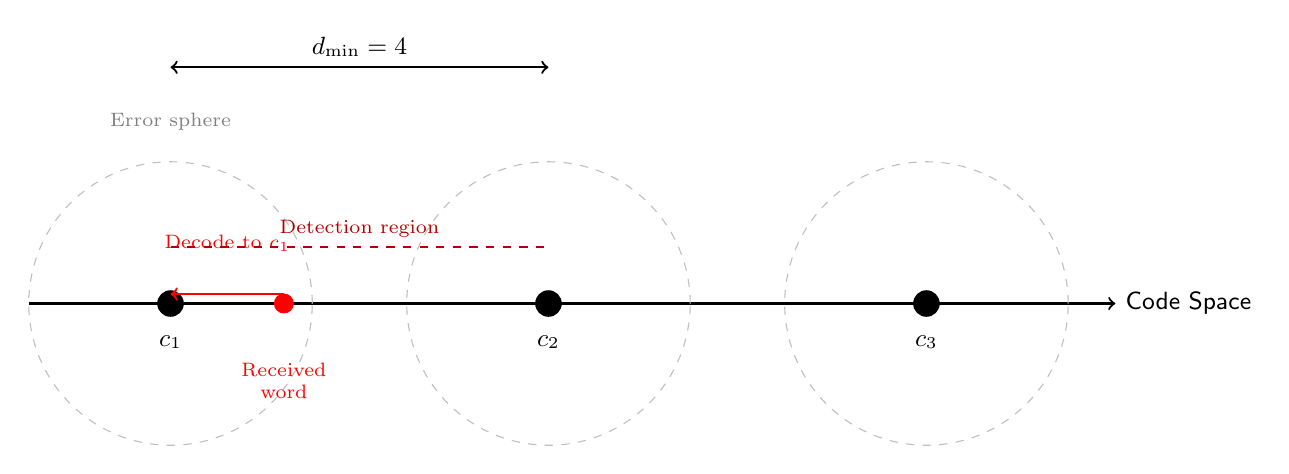
\begin{tikzpicture}[scale=1.2]
% Draw horizontal line representing code space
\draw[->,thick] (-0.5,0) -- (11,0) node[right] {\sffamily\small Code Space};

% Codeword 1
\fill[black] (1,0) circle (4pt);
\node[below=8pt] at (1,0) {\sffamily\small $c_1$};
\draw[dashed,gray!50] (1,0) circle (1.5cm);
\node[above=8pt,gray,font=\scriptsize] at (1,1.5) {Error sphere};

% Codeword 2
\fill[black] (5,0) circle (4pt);
\node[below=8pt] at (5,0) {\sffamily\small $c_2$};
\draw[dashed,gray!50] (5,0) circle (1.5cm);

% Codeword 3
\fill[black] (9,0) circle (4pt);
\node[below=8pt] at (9,0) {\sffamily\small $c_3$};
\draw[dashed,gray!50] (9,0) circle (1.5cm);

% Distance annotation
\draw[<->,thick] (1,2.5) -- (5,2.5) node[midway,above] {\sffamily\small $d_{\min} = 4$};

% Received word example
\fill[red] (2.2,0) circle (3pt);
\node[below=18pt,red,font=\scriptsize,align=center] at (2.2,0) {Received\\word};
\draw[->,red,thick] (2.2,0.1) -- (1,0.1);
\node[above=12pt,red,font=\scriptsize] at (1.6,0.1) {Decode to $c_1$};

% Error detection region
\draw[thick,red!70!black,dashed] (1,0.6) -- (5,0.6);
\node[above,red!70!black,font=\scriptsize] at (3,0.6) {Detection region};
\end{tikzpicture}
\end{center}

With $d_{\min} = 4$, the code can correct $t = \lfloor(4-1)/2\rfloor = 1$ error or detect up to $4-1 = 3$ errors. Error spheres of radius 1 (dashed circles) around each codeword remain disjoint.

\section{Code Examples}\label{examples}

\subsection{Simple Parity Code}

Add one parity bit to make the total number of 1's even (even parity) or odd (odd parity).

\textbf{Encoding (even parity):}
\begin{equation}
p = d_1 \oplus d_2 \oplus \cdots \oplus d_k
\label{eq:parity-even}
\end{equation}
where:
\begin{itemize}
\item $p$ = parity bit
\item $d_i$ = data bits ($i = 1, 2, \ldots, k$)
\item $\oplus$ = XOR (exclusive OR) operation
\end{itemize}

\textbf{Example (3-bit data):}
\begin{itemize}
\item $000 \rightarrow 000\mathbf{0}$ (0 ones, even)
\item $001 \rightarrow 001\mathbf{1}$ (2 ones, even)
\item $010 \rightarrow 010\mathbf{1}$ (2 ones, even)
\item $011 \rightarrow 011\mathbf{0}$ (2 ones, even)
\end{itemize}

\textbf{Code parameters:}
\begin{itemize}
\item $(n, k) = (k+1, k)$ (add 1 parity bit to $k$ data bits)
\item $d_{\min} = 2$ (any two codewords differ in $\geq 2$ positions)
\item Detection capability: $t_{\text{detect}} = 1$ error
\item Correction capability: $t_{\text{correct}} = 0$ errors
\item Code rate: $R = k/(k+1) \approx 0.875$ for $k=8$
\end{itemize}

\subsection{Repetition Code (3-bit)}

Repeat each bit $n$ times to create redundancy.

\textbf{Encoding for $(n, 1)$ repetition code:}
\begin{equation}
\text{Bit } 0 \rightarrow \underbrace{00\cdots0}_{n \text{ times}}, \quad \text{Bit } 1 \rightarrow \underbrace{11\cdots1}_{n \text{ times}}
\label{eq:repetition}
\end{equation}

\textbf{For $n = 3$:}
\begin{itemize}
\item Bit $0 \rightarrow 000$
\item Bit $1 \rightarrow 111$
\end{itemize}

\textbf{Code parameters:}
\begin{itemize}
\item $(n, k) = (3, 1)$
\item $d_{\min} = 3$ (codewords 000 and 111 differ in all 3 positions)
\item Detection capability: $t_{\text{detect}} = 2$ errors
\item Correction capability: $t_{\text{correct}} = 1$ error
\item Code rate: $R = 1/3 \approx 0.33$ (very inefficient)
\end{itemize}

\textbf{Decoding (majority vote):}
\begin{equation}
\hat{d} = \begin{cases}
0 & \text{if } w_H(\text{received}) \leq 1 \\
1 & \text{if } w_H(\text{received}) \geq 2
\end{cases}
\label{eq:majority-vote}
\end{equation}

\textbf{Example:} Received word $010$ (1 error) $\rightarrow$ Weight $= 1$ $\rightarrow$ Decode as bit 0 (codeword 000).

\subsection{Hamming(7,4) Code}

The Hamming(7,4) code is a perfect single-error-correcting code.

\textbf{Code parameters:}
\begin{itemize}
\item $(n, k) = (7, 4)$ (7 total bits: 4 data + 3 parity)
\item $d_{\min} = 3$
\item Detection capability: $t_{\text{detect}} = 2$ errors
\item Correction capability: $t_{\text{correct}} = 1$ error
\item Code rate: $R = 4/7 \approx 0.57$ (57\% data, 43\% overhead)
\end{itemize}

\textbf{Parity check equations:}
\begin{align}
p_1 &= d_1 \oplus d_2 \oplus d_4 \label{eq:hamming-p1} \\
p_2 &= d_1 \oplus d_3 \oplus d_4 \label{eq:hamming-p2} \\
p_3 &= d_2 \oplus d_3 \oplus d_4 \label{eq:hamming-p3}
\end{align}
where $d_1, d_2, d_3, d_4$ are data bits and $p_1, p_2, p_3$ are parity bits.

\textbf{Codeword structure:} $[p_1, p_2, d_1, p_3, d_2, d_3, d_4]$

The syndrome computed from the received word identifies the error position, enabling single-error correction.

\section{Hamming Weight and Linear Codes}

\subsection{Hamming Weight}

The Hamming weight of a binary string is the number of 1's (non-zero bits):
\begin{equation}
w_H(x) = \sum_{i=1}^{n} x_i
\label{eq:hamming-weight}
\end{equation}
where:
\begin{itemize}
\item $w_H(x)$ = Hamming weight of string $x$
\item $x_i \in \{0, 1\}$ = bits of string $x$
\end{itemize}

\textbf{Relationship between distance and weight:}
\begin{equation}
d_H(x, y) = w_H(x \oplus y)
\label{eq:distance-weight}
\end{equation}
where $\oplus$ denotes bitwise XOR (exclusive OR) operation.

\textbf{Example:}
\begin{align*}
x &= 10110 \\
y &= 10011 \\
x \oplus y &= 00101 \quad \text{(weight = 2)} \\
\therefore d_H(x, y) &= 2
\end{align*}

\subsection{Minimum Distance of Linear Codes}

For \textbf{linear codes} (codes closed under addition), the minimum distance equals the minimum non-zero codeword weight:
\begin{equation}
d_{\min} = \min_{\substack{c \in C \\ c \neq 0}} w_H(c)
\label{eq:linear-min-distance}
\end{equation}
where:
\begin{itemize}
\item $C$ = set of all codewords
\item $0$ = all-zero codeword
\end{itemize}

\textbf{Why this works:} For linear codes, $c_1 \oplus c_2$ is also a codeword. Therefore:
\[
d_H(c_1, c_2) = w_H(c_1 \oplus c_2) = w_H(c_3)
\]
where $c_3 = c_1 \oplus c_2 \in C$.

\begin{calloutbox}{Computational Advantage}
For a linear $(n,k)$ code with $2^k$ codewords, finding $d_{\min}$ by:
\begin{itemize}
\item \textbf{Pairwise comparison:} $\binom{2^k}{2} = O(2^{2k})$ comparisons
\item \textbf{Weight enumeration:} $2^k - 1$ weight calculations (excludes all-zero)
\end{itemize}

For Hamming(7,4): $\binom{16}{2} = 120$ vs $15$ calculations---8$\times$ faster!
\end{calloutbox}

\section{Error Detection and Correction Spheres}

The error-handling capability can be visualized using Hamming spheres around each codeword.

\begin{center}
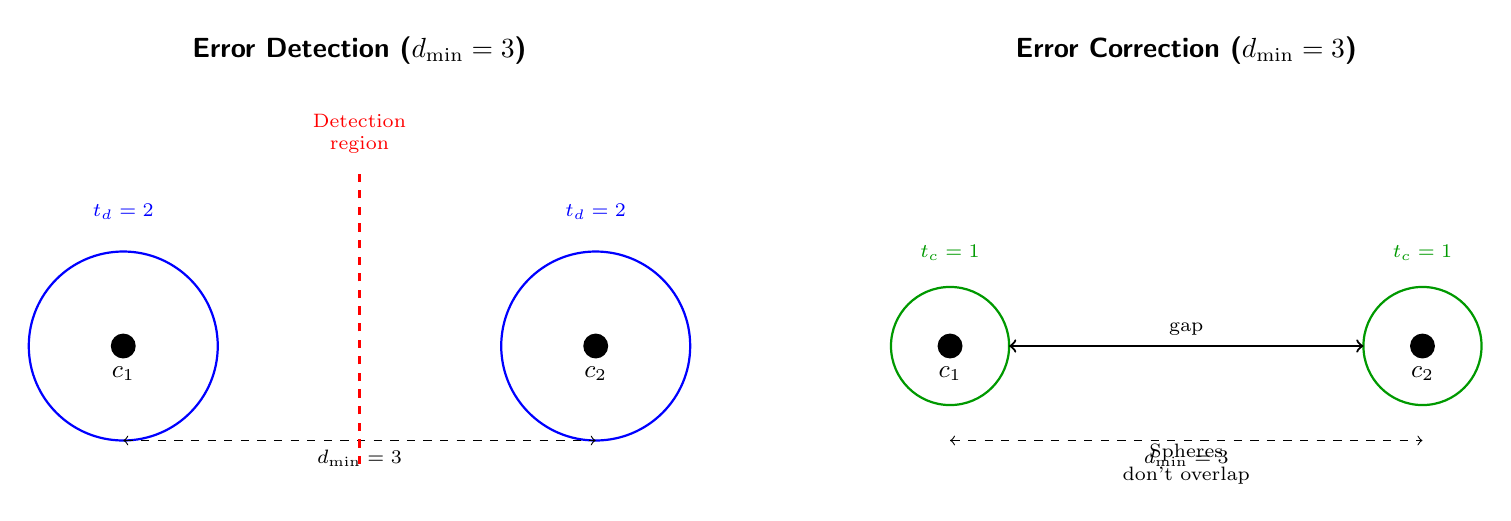
\begin{tikzpicture}[scale=1.5]
% Title annotations
\node[font=\sffamily\bfseries] at (3,3.5) {Error Detection ($d_{\min} = 3$)};
\node[font=\sffamily\bfseries] at (10,3.5) {Error Correction ($d_{\min} = 3$)};

% Left diagram - Detection only
\begin{scope}[shift={(0,0)}]
% Codeword 1
\fill[black] (1,1) circle (3pt);
\node[below=4pt,font=\small] at (1,1) {$c_1$};
\draw[thick,blue] (1,1) circle (0.8cm);
\node[above=8pt,blue,font=\scriptsize] at (1,1.8) {$t_d = 2$};

% Codeword 2
\fill[black] (5,1) circle (3pt);
\node[below=4pt,font=\small] at (5,1) {$c_2$};
\draw[thick,blue] (5,1) circle (0.8cm);
\node[above=8pt,blue,font=\scriptsize] at (5,1.8) {$t_d = 2$};

% Distance line
\draw[<->,dashed] (1,0.2) -- (5,0.2) node[midway,below,font=\scriptsize] {$d_{\min} = 3$};

% Detection region overlap
\draw[thick,red,dashed] (3,0) -- (3,2.5);
\node[red,font=\scriptsize,align=center] at (3,2.8) {Detection\\region};
\end{scope}

% Right diagram - Correction
\begin{scope}[shift={(7,0)}]
% Codeword 1
\fill[black] (1,1) circle (3pt);
\node[below=4pt,font=\small] at (1,1) {$c_1$};
\draw[thick,green!60!black] (1,1) circle (0.5cm);
\node[above=6pt,green!60!black,font=\scriptsize] at (1,1.5) {$t_c = 1$};

% Codeword 2
\fill[black] (5,1) circle (3pt);
\node[below=4pt,font=\small] at (5,1) {$c_2$};
\draw[thick,green!60!black] (5,1) circle (0.5cm);
\node[above=6pt,green!60!black,font=\scriptsize] at (5,1.5) {$t_c = 1$};

% Distance line
\draw[<->,dashed] (1,0.2) -- (5,0.2) node[midway,below,font=\scriptsize] {$d_{\min} = 3$};

% Gap between spheres
\draw[<->,thick] (1.5,1) -- (4.5,1) node[midway,above,font=\scriptsize] {gap};
\node[font=\scriptsize,align=center] at (3,0) {Spheres\\don't overlap};
\end{scope}
\end{tikzpicture}
\end{center}

\textbf{Left:} Detection spheres of radius $t_d = d_{\min} - 1 = 2$ extend to the midpoint between codewords. Any error within this radius is detected.

\textbf{Right:} Correction spheres of radius $t_c = \lfloor(d_{\min} - 1)/2\rfloor = 1$ remain disjoint, ensuring unique decoding to the nearest codeword.

\section{Error Detection Methods}\label{error-detection-methods}

\subsection{Single Parity Check}

Add one bit to make the total number of 1's even (or odd).

\textbf{Even parity encoding:}
\begin{equation}
p = d_1 \oplus d_2 \oplus \cdots \oplus d_k = \bigoplus_{i=1}^{k} d_i
\label{eq:single-parity}
\end{equation}

\textbf{Properties:}
\begin{itemize}
\item $d_{\min} = 2$
\item Detects \textbf{all single-bit errors}
\item Detects \textbf{all odd-number errors} (1, 3, 5, \ldots)
\item \textbf{Cannot detect even-number errors} (2, 4, 6, \ldots)
\item Overhead: 1 bit per $k$ data bits ($\sim$12.5\% for $k=8$)
\end{itemize}

\textbf{Use cases:} Memory modules (SIMM, DIMM), serial communication (UART parity bit)

\subsubsection{2. Two-Dimensional Parity}\label{two-dimensional-parity}

\textbf{Arrange data in matrix}, add parity for rows and columns:

\begin{verbatim}
d11  d12  d13  | p1  (row parity)
d21  d22  d23  | p2
d31  d32  d33  | p3
-----------------
 c1   c2   c3  | pc  (col parity, overall)
\end{verbatim}

\textbf{Properties}: - Detect all 1, 2, 3-bit errors - Correct
single-bit error (row \$\textbackslash cap\$ column identifies position)
- Some 4+ bit error patterns undetected

\begin{center}\rule{0.5\linewidth}{0.5pt}\end{center}

\subsection{Cyclic Redundancy Check (CRC)}

Polynomial-based error detection treating the message as a polynomial over GF(2).

\textbf{Encoding procedure:}
\begin{equation}
\text{CRC}(m) = m(x) \cdot x^r \bmod g(x)
\label{eq:crc-encoding}
\end{equation}
where:
\begin{itemize}
\item $m(x)$ = message polynomial
\item $g(x)$ = generator polynomial of degree $r$
\item $r$ = number of CRC bits
\item $\bmod$ = polynomial modulo (remainder after division)
\end{itemize}

\textbf{Transmitted codeword:}
\begin{equation}
c(x) = m(x) \cdot x^r + \text{CRC}(m)
\label{eq:crc-codeword}
\end{equation}

\textbf{Example (CRC-8):}
\begin{itemize}
\item Generator: $g(x) = x^8 + x^2 + x + 1$ (binary: 100000111)
\item Produces 8-bit checksum
\end{itemize}

\textbf{Detection properties:}
\begin{itemize}
\item Detects \textbf{all single-bit errors}
\item Detects \textbf{all double-bit errors}
\item Detects \textbf{all odd-number errors} (if $g(x)$ has $(x+1)$ factor)
\item Detects \textbf{all burst errors} $\leq$ degree of $g(x)$
\item Detects $(1 - 2^{-r})$ of longer burst errors
\end{itemize}

\textbf{Common CRC standards:}
\begin{itemize}
\item \textbf{CRC-16} (16 bits): Modbus, USB 2.0
\item \textbf{CRC-32} (32 bits): Ethernet, ZIP, PNG, MPEG-2
\item \textbf{CRC-CCITT} (16 bits): Bluetooth, X.25, HDLC
\end{itemize}

\subsection{Checksum}

Simple sum of data bytes with wraparound, commonly used in network protocols.

\textbf{16-bit checksum computation:}
\begin{equation}
\text{Checksum} = \left(-\sum_{i} \text{data}_i\right) \bmod 2^{16}
\label{eq:checksum}
\end{equation}

\textbf{Properties:}
\begin{itemize}
\item Very fast to compute (simple addition)
\item Weaker than CRC (doesn't catch all bit reorderings)
\item Commonly used when computational simplicity is critical
\end{itemize}

\textbf{Use cases:} TCP, UDP, IP headers (IPv4 header checksum)

\subsection{Error Correction
Principles}\label{error-correction-principles}

\subsubsection{Maximum Likelihood
Decoding}\label{maximum-likelihood-decoding}

\textbf{Receive} \(r\) (possibly corrupted)

\textbf{Decode to codeword} \(\hat{c}\) that maximizes \(P(c | r)\)

\textbf{For AWGN channel}: Minimum Euclidean distance

\textbf{For BSC} (binary symmetric channel): Minimum Hamming distance

\[
\hat{c} = \arg\min_{c \in C} d_H(r, c)
\]

\begin{center}\rule{0.5\linewidth}{0.5pt}\end{center}

\subsubsection{Syndrome Decoding}\label{syndrome-decoding}

\textbf{For linear codes}:

\textbf{Syndrome}: \(s = r \cdot H^T\)

Where: - \(r\) = Received word - \(H\) = Parity-check matrix

\textbf{Property}: \(s = 0\) iff \(r\) is valid codeword

\textbf{Error pattern} identified by syndrome lookup table

\begin{center}\rule{0.5\linewidth}{0.5pt}\end{center}

\subsubsection{Bounded Distance
Decoding}\label{bounded-distance-decoding}

\textbf{Decode successfully if} \(d_H(r, c) \leq t\)

Where \(t = \lfloor (d_{\min} - 1)/2 \rfloor\)

\textbf{If} \(d_H(r, c) > t\) \textbf{for all} \(c\): -
\textbf{Erasure}: Declare decoding failure (more honest) -
\textbf{Guess}: Pick nearest (may introduce errors)

\begin{center}\rule{0.5\linewidth}{0.5pt}\end{center}

\section{Coding Bounds}

\subsection{Hamming Bound (Sphere-Packing Bound)}

The volume of a Hamming sphere of radius $t$ (number of words within distance $t$ of a center):
\begin{equation}
V(t) = \sum_{i=0}^{t} \binom{n}{i}
\label{eq:sphere-volume}
\end{equation}
where:
\begin{itemize}
\item $n$ = codeword length
\item $t$ = sphere radius (error correction capability)
\item $\binom{n}{i}$ = number of words at distance exactly $i$
\end{itemize}

\textbf{Hamming bound:} For an $(n, k)$ code correcting $t$ errors:
\begin{equation}
2^k \cdot V(t) \leq 2^n
\label{eq:hamming-bound}
\end{equation}

Equivalently (number of parity bits):
\begin{equation}
2^{n-k} \geq \sum_{i=0}^{t} \binom{n}{i}
\label{eq:hamming-bound-parity}
\end{equation}

\textbf{Interpretation:} The $2^k$ codewords, each with a sphere of radius $t$, must fit within the total space of $2^n$ possible $n$-bit words. This bound limits how many parity bits are needed for a given error correction capability.

\subsubsection{Perfect Codes}\label{perfect-codes}

\textbf{Code is perfect} if Hamming bound is met with equality

\textbf{Examples}: - Hamming codes (single-error correcting) - Golay
code (23, 12, 7) - Repetition codes (trivial)

\textbf{Property}: Every received word is within distance \(t\) of
exactly one codeword (no ``wasted'' space)

\begin{center}\rule{0.5\linewidth}{0.5pt}\end{center}

\subsubsection{Singleton Bound}\label{singleton-bound}

\[
d_{\min} \leq n - k + 1
\]

\textbf{Codes meeting this}: \textbf{Maximum Distance Separable (MDS)}

\textbf{Examples}: Reed-Solomon codes (meet Singleton bound)

\begin{center}\rule{0.5\linewidth}{0.5pt}\end{center}

\subsubsection{Gilbert-Varshamov Bound}\label{gilbert-varshamov-bound}

\textbf{Existence bound}: Guarantees codes exist with certain
\(d_{\min}\)

\[
\sum_{i=0}^{d-2} \binom{n-1}{i} < 2^{n-k}
\]

\textbf{Interpretation}: ``Good'' codes exist, even if we
don\textquotesingle t know how to construct them

\begin{center}\rule{0.5\linewidth}{0.5pt}\end{center}

\subsection{Practical Error Detection}\label{practical-error-detection}

\subsubsection{Memory (ECC RAM)}\label{memory-ecc-ram}

\textbf{Single Error Correction, Double Error Detection (SECDED)}: -
Hamming code with extra parity bit - \(d_{\min} = 4\) - Correct 1 bit,
detect 2 bits

\textbf{Example}: 64-bit data - Hamming: 7 parity bits (for 1-bit
correction) - +1 bit for double detection \$\textbackslash rightarrow\$
8 bits total - (64, 72) SECDED code

\begin{center}\rule{0.5\linewidth}{0.5pt}\end{center}

\subsubsection{Storage (Hard Drives,
SSDs)}\label{storage-hard-drives-ssds}

\textbf{Reed-Solomon codes}: - Detect/correct burst errors - Used in
RAID, CDs, DVDs, QR codes

\textbf{Example}: CD - RS(32, 28, 5) over \(\mathrm{GF}(2^8)\) - Can
correct 2 symbol errors (16 bits)

\begin{center}\rule{0.5\linewidth}{0.5pt}\end{center}

\subsubsection{Networking}\label{networking}

\textbf{CRC-32} (Ethernet): - Detects all burst errors
\$\textbackslash leq\$32 bits - Detects 99.9999\% of longer bursts

\textbf{TCP checksum}: - 16-bit sum (weak) - Mainly detects random
errors, not malicious

\begin{center}\rule{0.5\linewidth}{0.5pt}\end{center}

\subsubsection{Spacecraft}\label{spacecraft}

\textbf{Concatenated codes}: - Inner: Convolutional or LDPC (correct
frequent errors) - Outer: Reed-Solomon (correct burst errors)

\textbf{Example}: Voyager - (7, 1/2) convolutional + RS(255, 223) -
\(d_{\min} = 33\) (outer code) - Can correct 16 symbol errors

\begin{center}\rule{0.5\linewidth}{0.5pt}\end{center}

\subsection{Burst Error Detection}\label{burst-error-detection}

\textbf{Burst error}: Consecutive bits corrupted

\textbf{Length \(b\) burst}: Errors span \(b\) consecutive bits

\begin{center}\rule{0.5\linewidth}{0.5pt}\end{center}

\subsubsection{Fire Codes}\label{fire-codes}

\textbf{Designed for burst errors}

\textbf{Parameters}: \((n, k)\) code detecting bursts
\$\textbackslash leq\$ \(b\)

\textbf{Requirement}: \(n - k \geq b\)

\textbf{Generator polynomial}: Special structure

\begin{center}\rule{0.5\linewidth}{0.5pt}\end{center}

\subsubsection{Interleaving}\label{interleaving}

\textbf{Spread codeword symbols} across time/space

\textbf{Example (depth 5)}:

\begin{verbatim}
Original:
C1: a1 a2 a3 a4
C2: b1 b2 b3 b4
C3: c1 c2 c3 c4
C4: d1 d2 d3 d4
C5: e1 e2 e3 e4

Transmitted:
a1 b1 c1 d1 e1 | a2 b2 c2 d2 e2 | a3 b3 c3 d3 e3 | ...

If burst corrupts 5 bits:
a1 b1 c1 d1 e1  (all corrupted)
         
Each codeword sees only 1 error  All correctable!
\end{verbatim}

\textbf{Use case}: CDs (scratch protection), wireless (fading)

\begin{center}\rule{0.5\linewidth}{0.5pt}\end{center}

\subsection{Distance Spectrum}\label{distance-spectrum}

\textbf{Weight distribution} \(A_i\) = Number of codewords with weight
\(i\)

\textbf{Notation}: \(\{A_0, A_1, A_2, \ldots, A_n\}\)

\textbf{Example}: Hamming(7,4) - \(A_0 = 1\) (all-zeros) - \(A_3 = 7\)
(weight 3) - \(A_4 = 7\) (weight 4) - \(A_7 = 1\) (all-ones)

\textbf{Use}: Calculate average error probability

\begin{center}\rule{0.5\linewidth}{0.5pt}\end{center}

\subsubsection{Union Bound on Error
Probability}\label{union-bound-on-error-probability}

\[
P_e \leq \sum_{i=d_{\min}}^{n} A_i \cdot P(\text{decode } c_i \text{ as another codeword})
\]

\textbf{Tight at high SNR}

\begin{center}\rule{0.5\linewidth}{0.5pt}\end{center}

\subsection{Soft-Decision Metrics}\label{soft-decision-metrics}

\textbf{Hard decision}: Received bit \$\textbackslash rightarrow\$ 0 or
1 (threshold)

\textbf{Soft decision}: Keep analog value (confidence)

\textbf{Soft Hamming distance} (Euclidean):

\[
d_{\text{soft}}(r, c) = \sum_{i=1}^{n} (r_i - c_i)^2
\]

Where \(r_i \in \mathbb{R}\) (e.g., LLRs)

\textbf{Benefit}: \textasciitilde2-3 dB coding gain

\begin{center}\rule{0.5\linewidth}{0.5pt}\end{center}

\subsection{Summary Table}\label{summary-table}

{\def\LTcaptype{} % do not increment counter
\begin{longtable}[]{@{}llll@{}}
\toprule\noalign{}
Error Type & Detection Method & Overhead & Capability \\
\midrule\noalign{}
\endhead
\bottomrule\noalign{}
\endlastfoot
\textbf{Single bit} & Parity & 1 bit & Detect only \\
\textbf{1-2 bits} & Hamming(7,4) & 43\% & Correct 1, detect 2 \\
\textbf{Burst \$\textbackslash leq\$32 bits} & CRC-32 & 32 bits & Detect
only \\
\textbf{Random errors} & Reed-Solomon & 10-20\% & Correct + detect \\
\textbf{Deep space} & Concatenated & 50\%+ & Very robust \\
\end{longtable}
}

\begin{center}\rule{0.5\linewidth}{0.5pt}\end{center}

\subsection{Code Comparison}\label{code-comparison}

{\def\LTcaptype{} % do not increment counter
\begin{longtable}[]{@{}llllll@{}}
\toprule\noalign{}
Code & (n, k) & \(d_{\min}\) & Correct & Detect & Rate \\
\midrule\noalign{}
\endhead
\bottomrule\noalign{}
\endlastfoot
\textbf{Parity} & (n, n-1) & 2 & 0 & 1 & 0.875 (n=8) \\
\textbf{Rep(3)} & (3, 1) & 3 & 1 & 2 & 0.33 \\
\textbf{Hamming(7,4)} & (7, 4) & 3 & 1 & 2 & 0.57 \\
\textbf{Extended Hamming} & (8, 4) & 4 & 1 & 3 & 0.50 \\
\textbf{Golay(23,12)} & (23, 12) & 7 & 3 & 6 & 0.52 \\
\textbf{RS(255,223)} & (255, 223) & 33 & 16 & 32 & 0.875 \\
\end{longtable}
}

\begin{center}\rule{0.5\linewidth}{0.5pt}\end{center}

\subsection{Python Example: Hamming
Distance}\label{python-example-hamming-distance}

\begin{Shaded}
\begin{Highlighting}[]
\KeywordTok{def}\NormalTok{ hamming\_distance(x, y):}
    \CommentTok{"""Calculate Hamming distance between two binary strings."""}
    \ControlFlowTok{if} \BuiltInTok{len}\NormalTok{(x) }\OperatorTok{!=} \BuiltInTok{len}\NormalTok{(y):}
        \ControlFlowTok{raise} \PreprocessorTok{ValueError}\NormalTok{(}\StringTok{"Strings must have equal length"}\NormalTok{)}
    \ControlFlowTok{return} \BuiltInTok{sum}\NormalTok{(c1 }\OperatorTok{!=}\NormalTok{ c2 }\ControlFlowTok{for}\NormalTok{ c1, c2 }\KeywordTok{in} \BuiltInTok{zip}\NormalTok{(x, y))}

\KeywordTok{def}\NormalTok{ hamming\_weight(x):}
    \CommentTok{"""Calculate Hamming weight (number of 1\textquotesingle{}s)."""}
    \ControlFlowTok{return} \BuiltInTok{sum}\NormalTok{(}\BuiltInTok{int}\NormalTok{(c) }\ControlFlowTok{for}\NormalTok{ c }\KeywordTok{in}\NormalTok{ x)}

\KeywordTok{def}\NormalTok{ minimum\_distance(codewords):}
    \CommentTok{"""Find minimum distance of a code."""}
\NormalTok{    min\_dist }\OperatorTok{=} \BuiltInTok{float}\NormalTok{(}\StringTok{\textquotesingle{}inf\textquotesingle{}}\NormalTok{)}
    \ControlFlowTok{for}\NormalTok{ i, c1 }\KeywordTok{in} \BuiltInTok{enumerate}\NormalTok{(codewords):}
        \ControlFlowTok{for}\NormalTok{ c2 }\KeywordTok{in}\NormalTok{ codewords[i}\OperatorTok{+}\DecValTok{1}\NormalTok{:]:}
\NormalTok{            dist }\OperatorTok{=}\NormalTok{ hamming\_distance(c1, c2)}
            \ControlFlowTok{if}\NormalTok{ dist }\OperatorTok{\textless{}}\NormalTok{ min\_dist:}
\NormalTok{                min\_dist }\OperatorTok{=}\NormalTok{ dist}
    \ControlFlowTok{return}\NormalTok{ min\_dist}

\CommentTok{\# Example: Hamming(7,4) codewords}
\NormalTok{hamming\_7\_4 }\OperatorTok{=}\NormalTok{ [}
    \StringTok{\textquotesingle{}0000000\textquotesingle{}}\NormalTok{, }\StringTok{\textquotesingle{}0001111\textquotesingle{}}\NormalTok{, }\StringTok{\textquotesingle{}0010110\textquotesingle{}}\NormalTok{, }\StringTok{\textquotesingle{}0011001\textquotesingle{}}\NormalTok{,}
    \StringTok{\textquotesingle{}0100101\textquotesingle{}}\NormalTok{, }\StringTok{\textquotesingle{}0101010\textquotesingle{}}\NormalTok{, }\StringTok{\textquotesingle{}0110011\textquotesingle{}}\NormalTok{, }\StringTok{\textquotesingle{}0111100\textquotesingle{}}\NormalTok{,}
    \StringTok{\textquotesingle{}1000011\textquotesingle{}}\NormalTok{, }\StringTok{\textquotesingle{}1001100\textquotesingle{}}\NormalTok{, }\StringTok{\textquotesingle{}1010101\textquotesingle{}}\NormalTok{, }\StringTok{\textquotesingle{}1011010\textquotesingle{}}\NormalTok{,}
    \StringTok{\textquotesingle{}1100110\textquotesingle{}}\NormalTok{, }\StringTok{\textquotesingle{}1101001\textquotesingle{}}\NormalTok{, }\StringTok{\textquotesingle{}1110000\textquotesingle{}}\NormalTok{, }\StringTok{\textquotesingle{}1111111\textquotesingle{}}
\NormalTok{]}

\NormalTok{d\_min }\OperatorTok{=}\NormalTok{ minimum\_distance(hamming\_7\_4)}
\BuiltInTok{print}\NormalTok{(}\SpecialStringTok{f"Minimum distance: }\SpecialCharTok{\{}\NormalTok{d\_min}\SpecialCharTok{\}}\SpecialStringTok{"}\NormalTok{)  }\CommentTok{\# Output: 3}

\CommentTok{\# Error capability}
\NormalTok{t\_correct }\OperatorTok{=}\NormalTok{ (d\_min }\OperatorTok{{-}} \DecValTok{1}\NormalTok{) }\OperatorTok{//} \DecValTok{2}
\NormalTok{t\_detect }\OperatorTok{=}\NormalTok{ d\_min }\OperatorTok{{-}} \DecValTok{1}
\BuiltInTok{print}\NormalTok{(}\SpecialStringTok{f"Can correct }\SpecialCharTok{\{}\NormalTok{t\_correct}\SpecialCharTok{\}}\SpecialStringTok{ errors, detect }\SpecialCharTok{\{}\NormalTok{t\_detect}\SpecialCharTok{\}}\SpecialStringTok{ errors"}\NormalTok{)}
\CommentTok{\# Output: Can correct 1 errors, detect 2 errors}
\end{Highlighting}
\end{Shaded}

\begin{center}\rule{0.5\linewidth}{0.5pt}\end{center}

\section{Worked Example: Code Selection for Data Storage}

\textbf{Problem:} Design an error control scheme for a data storage system that must protect 64-bit data words against cosmic ray-induced bit flips.

\subsection*{Given Parameters}

\begin{tabular}{@{}ll@{}}
Data word size & $k = 64$ bits \\
Required capability & Correct 1 error, detect 2 errors (SECDED) \\
Channel & Single-bit errors (cosmic rays) \\
Maximum overhead & 20\% (12.8 additional bits) \\
\end{tabular}

\subsection*{Required}

Find:
\begin{enumerate}
\item Minimum distance $d_{\min}$ required
\item Number of parity bits needed
\item Suitable code selection
\item Verify using Hamming bound
\end{enumerate}

\subsection*{Solution}

\textbf{Step 1: Determine required minimum distance}

Using Equation~\ref{eq:combined-capability} for combined correction/detection:
\begin{equation}
d_{\min} \geq 2t + s + 1
\end{equation}

For $t = 1$ (correct 1 error) and $s = 1$ (detect 1 additional error beyond correction):
\begin{equation}
d_{\min} \geq 2(1) + 1 + 1 = 4
\end{equation}

\textbf{Answer:} Need $d_{\min} = 4$ for SECDED capability.

\textbf{Step 2: Estimate parity bits using Hamming bound}

From Equation~\ref{eq:hamming-bound-parity} for $t = 1$ correction:
\begin{equation}
2^{n-k} \geq \sum_{i=0}^{1} \binom{n}{i} = 1 + n
\end{equation}

With $k = 64$ and $n = k + r$ where $r$ is parity bits:
\begin{equation}
2^r \geq 1 + 64 + r
\end{equation}

Testing values:
\begin{itemize}
\item $r = 6$: $2^6 = 64 < 71$ (fails)
\item $r = 7$: $2^7 = 128 > 72$ (passes)
\end{itemize}

Extended Hamming code adds 1 parity bit: $r = 7 + 1 = 8$ bits.

\textbf{Step 3: Verify overhead constraint}

\begin{equation}
\text{Overhead} = \frac{r}{k} = \frac{8}{64} = 0.125 = 12.5\%
\end{equation}

Since $12.5\% < 20\%$, the constraint is satisfied.

\textbf{Step 4: Code selection}

Use \textbf{Extended Hamming (72, 64) SECDED code}:
\begin{itemize}
\item $(n, k) = (72, 64)$ (8 parity bits)
\item $d_{\min} = 4$
\item Corrects 1 error: $t_c = \lfloor(4-1)/2\rfloor = 1$
\item Detects 2 errors: $t_d = 4 - 1 = 3$ (but we use 2 for SECDED mode)
\item Code rate: $R = 64/72 = 0.889$
\end{itemize}

\begin{calloutbox}{Design Verification}
\textbf{Performance summary:}
\begin{itemize}
\item \textbf{1 error:} Corrected automatically (no data loss)
\item \textbf{2 errors:} Detected but not corrected (system alerts/retries)
\item \textbf{3+ errors:} May be undetected (probability $< 10^{-10}$ for cosmic rays)
\end{itemize}

\textbf{Real-world usage:} This (72,64) SECDED scheme is the standard ECC implementation in DDR4 and DDR5 memory modules.
\end{calloutbox}

\subsection*{Visualization of Code Selection}

\begin{center}
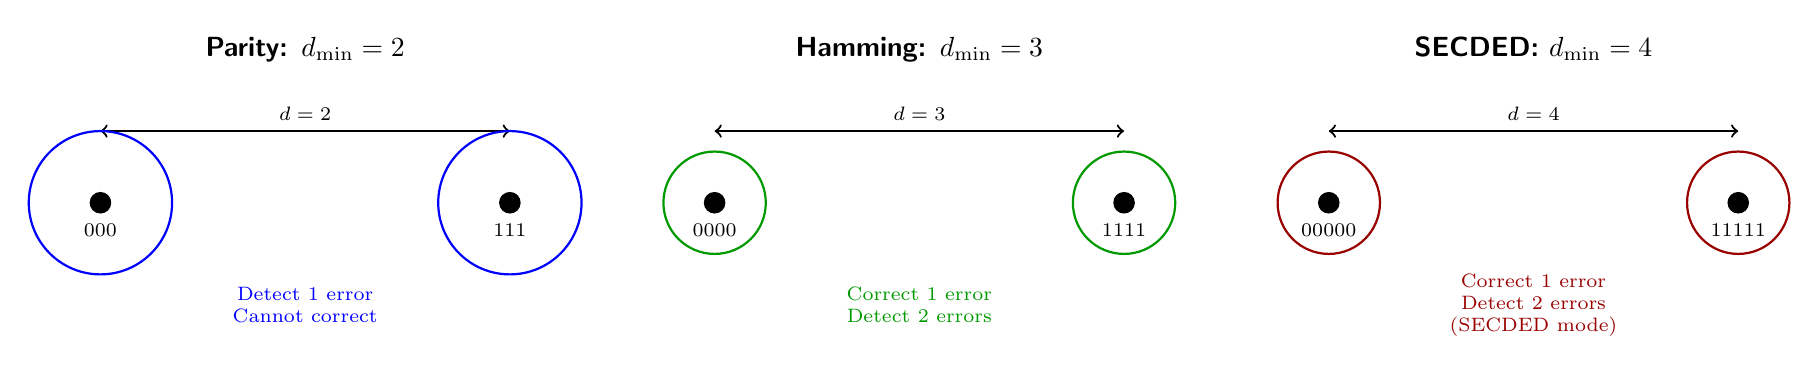
\begin{tikzpicture}[scale=1.3]
% Three code examples showing tradeoffs
% Parity code
\begin{scope}[shift={(0,0)}]
\node[font=\sffamily\bfseries] at (2,3) {Parity: $d_{\min}=2$};
\fill[black] (0,1.5) circle (3pt);
\node[below=4pt,font=\scriptsize] at (0,1.5) {000};
\fill[black] (4,1.5) circle (3pt);
\node[below=4pt,font=\scriptsize] at (4,1.5) {111};
\draw[<->,thick] (0,2.2) -- (4,2.2) node[midway,above,font=\scriptsize] {$d=2$};
\draw[blue,thick] (0,1.5) circle (0.7cm);
\draw[blue,thick] (4,1.5) circle (0.7cm);
\node[blue,font=\scriptsize,align=center] at (2,0.5) {Detect 1 error\\Cannot correct};
\end{scope}

% Hamming code
\begin{scope}[shift={(6,0)}]
\node[font=\sffamily\bfseries] at (2,3) {Hamming: $d_{\min}=3$};
\fill[black] (0,1.5) circle (3pt);
\node[below=4pt,font=\scriptsize] at (0,1.5) {0000};
\fill[black] (4,1.5) circle (3pt);
\node[below=4pt,font=\scriptsize] at (4,1.5) {1111};
\draw[<->,thick] (0,2.2) -- (4,2.2) node[midway,above,font=\scriptsize] {$d=3$};
\draw[green!60!black,thick] (0,1.5) circle (0.5cm);
\draw[green!60!black,thick] (4,1.5) circle (0.5cm);
\node[green!60!black,font=\scriptsize,align=center] at (2,0.5) {Correct 1 error\\Detect 2 errors};
\end{scope}

% SECDED code
\begin{scope}[shift={(12,0)}]
\node[font=\sffamily\bfseries] at (2,3) {SECDED: $d_{\min}=4$};
\fill[black] (0,1.5) circle (3pt);
\node[below=4pt,font=\scriptsize] at (0,1.5) {00000};
\fill[black] (4,1.5) circle (3pt);
\node[below=4pt,font=\scriptsize] at (4,1.5) {11111};
\draw[<->,thick] (0,2.2) -- (4,2.2) node[midway,above,font=\scriptsize] {$d=4$};
\draw[red!60!black,thick] (0,1.5) circle (0.5cm);
\draw[red!60!black,thick] (4,1.5) circle (0.5cm);
\node[red!60!black,font=\scriptsize,align=center] at (2,0.5) {Correct 1 error\\Detect 2 errors\\(SECDED mode)};
\end{scope}
\end{tikzpicture}
\end{center}

As $d_{\min}$ increases, error protection improves but so does overhead. The optimal choice depends on application requirements.

\section{Bit Error Rate Performance}

The bit error rate (BER) improvement from error correction coding depends on the channel characteristics and code parameters.

\subsection{Uncoded Binary Symmetric Channel}

For a binary symmetric channel (BSC) with bit error probability $p$:
\begin{equation}
P_{\text{bit,uncoded}} = p
\label{eq:ber-uncoded}
\end{equation}

\subsection{Coded Performance}

For a code correcting up to $t$ errors over block length $n$:
\begin{equation}
P_{\text{block}} = \sum_{i=t+1}^{n} \binom{n}{i} p^i (1-p)^{n-i}
\label{eq:block-error}
\end{equation}
where:
\begin{itemize}
\item $P_{\text{block}}$ = probability of block decoding failure
\item $p$ = channel bit error probability
\item $t$ = error correction capability
\end{itemize}

\textbf{Approximation for $p \ll 1$:}
\begin{equation}
P_{\text{block}} \approx \binom{n}{t+1} p^{t+1}
\label{eq:block-error-approx}
\end{equation}

\subsection{Coding Gain Example}

Consider Hamming(7,4) code with $d_{\min} = 3$, $t = 1$:

At channel BER $p = 10^{-3}$:
\begin{itemize}
\item \textbf{Uncoded:} $P_{\text{bit}} = 10^{-3}$
\item \textbf{Coded:} $P_{\text{block}} \approx \binom{7}{2} (10^{-3})^2 = 21 \times 10^{-6}$
\item \textbf{Coding gain:} $10^{-3} / (21 \times 10^{-6}) \approx 48\times$ better
\end{itemize}

\begin{warningbox}
Coding introduces overhead that reduces effective data rate by factor $R = k/n$. For Hamming(7,4), $R = 4/7 = 0.57$, meaning only 57\% of transmitted bits are data. System designers must balance error protection against throughput reduction.
\end{warningbox}

\section{Applications}

\subsection{Memory Systems (ECC RAM)}

\textbf{Implementation:} Extended Hamming (72,64) SECDED code
\begin{itemize}
\item \textbf{Standard:} JEDEC DDR4/DDR5 specification
\item \textbf{Protection:} Corrects single-bit errors, detects double-bit errors
\item \textbf{Latency:} $<$1 ns encoding/decoding penalty
\item \textbf{Use case:} Server memory, mission-critical systems
\end{itemize}

\textbf{Performance:} Reduces uncorrectable error rate from $\sim$10 FIT to $<$0.1 FIT per Gb.

\subsection{Storage Systems}

\textbf{Hard Disk Drives (HDD):} Reed-Solomon codes
\begin{itemize}
\item \textbf{Code:} RS(255,239) over GF($2^8$)
\item \textbf{Parameters:} $d_{\min} = 17$, corrects 8 symbol (byte) errors
\item \textbf{Overhead:} 6.7\% (16 parity bytes per 239 data bytes)
\item \textbf{Sector format:} 512 bytes data + 40 bytes ECC
\end{itemize}

\textbf{Solid State Drives (SSD):} BCH codes + LDPC
\begin{itemize}
\item \textbf{Inner code:} BCH for wear-leveling errors
\item \textbf{Outer code:} LDPC for soft-decision decoding
\item \textbf{Overhead:} 15--25\% depending on endurance requirements
\end{itemize}

\subsection{Networking}

\textbf{Ethernet (IEEE 802.3):} CRC-32
\begin{itemize}
\item \textbf{Polynomial:} $g(x) = x^{32} + x^{26} + x^{23} + \cdots + 1$
\item \textbf{Frame Check Sequence:} 32-bit CRC appended to each frame
\item \textbf{Detection:} All burst errors $\leq 32$ bits, 99.9999\% of longer bursts
\item \textbf{Throughput:} Negligible overhead (32 bits per 1500-byte frame $=$ 0.3\%)
\end{itemize}

\textbf{Wi-Fi (IEEE 802.11):} Convolutional codes + CRC
\begin{itemize}
\item \textbf{PHY layer:} Rate 1/2 or 3/4 convolutional code
\item \textbf{MAC layer:} CRC-32 for error detection
\item \textbf{ARQ:} Retransmission if CRC fails
\end{itemize}

\subsection{Space Communications}

\textbf{Deep Space Network:} Concatenated codes
\begin{itemize}
\item \textbf{Inner code:} Rate 1/2 convolutional or LDPC
\item \textbf{Outer code:} Reed-Solomon RS(255,223)
\item \textbf{Interleaving:} Depth 4--8 to combat burst errors
\item \textbf{Coding gain:} 10--12 dB compared to uncoded
\end{itemize}

\textbf{Example:} Mars Reconnaissance Orbiter
\begin{itemize}
\item Data rate: 6 Mbps (maximum)
\item Code: Turbo code (rate 1/6) + RS(255,223)
\item Effective $d_{\min}$: Very large (approaching Shannon limit)
\end{itemize}

\section{Summary}

\begin{center}
\begin{tabular}{@{}ll@{}}
\toprule
\textbf{Concept} & \textbf{Description} \\
\midrule
Hamming distance & Number of bit positions where two words differ \\
Minimum distance & Smallest distance between any two codewords \\
Detection capability & $t_d = d_{\min} - 1$ errors \\
Correction capability & $t_c = \lfloor(d_{\min} - 1)/2\rfloor$ errors \\
Combined mode & Correct $t$ and detect $s$ if $d_{\min} \geq 2t + s + 1$ \\
Hamming weight & Number of 1's in a binary word \\
Linear code property & $d_{\min} = $ minimum non-zero weight \\
\midrule
\textbf{Common Codes} & \\
\midrule
Parity & $d_{\min} = 2$, detect 1 error \\
Hamming(7,4) & $d_{\min} = 3$, correct 1 error \\
Extended Hamming(8,4) & $d_{\min} = 4$, SECDED \\
CRC-32 & Detect burst errors $\leq 32$ bits \\
Reed-Solomon & MDS codes, optimal for burst errors \\
\bottomrule
\end{tabular}
\end{center}

\begin{keyconcept}
\textbf{Fundamental trade-off:} Larger $d_{\min}$ provides better error protection but requires more redundancy (lower code rate $R = k/n$). Optimal code selection balances error protection against overhead for the specific application.
\end{keyconcept}

\section{Further Reading}

\begin{itemize}
\item \textbf{Chapter 2:} Binary Symmetric Channel---theoretical foundation
\item \textbf{Chapter 8:} Forward Error Correction (FEC)---coding overview
\item \textbf{Chapter 9:} Block Codes (Hamming, BCH, Reed-Solomon)---specific constructions
\item \textbf{Chapter 10:} Convolutional Codes \& Viterbi Decoding---sequential codes
\item \textbf{Chapter 11:} LDPC Codes---modern capacity-approaching codes
\item \textbf{Chapter 15:} Bit Error Rate (BER) Analysis---performance metrics
\item \textbf{Chapter 20:} Interleaving Techniques---burst error mitigation
\end{itemize}
